\documentclass{standalone}
\usepackage{tikz}
\begin{document}

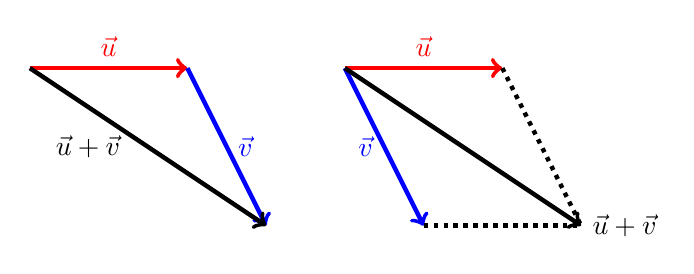
\begin{tikzpicture}[ultra thick]
  \draw[->, red](-1,0)-- node[above]{$\vec u$} (1,0);
  \draw[->, blue](1,0)-- node[right]{$\vec v$} (2,-2);
  \draw[->](-1,0)-- node[left, shift={(-6pt,0)}]{$\vec u + \vec v$} (2,-2);

\begin{scope}[shift={(4cm,0)}]
   \draw[->, red](-1,0)-- node[above]{$\vec u$} (1,0);
   \draw[->, blue](-1,0)--node[left]{$\vec v$}  (0,-2);
   \draw[dotted](1,0)--  (2,-2);
   \draw[dotted](0,-2)-- (2,-2);

   \draw[->](-1,0)-- (2,-2)node[right]{$\vec u + \vec v$} ;
\end{scope}

\end{tikzpicture}

\end{document}